\documentclass{article}

\usepackage{amsthm}
\usepackage{amsmath}
\usepackage{amssymb}
\usepackage{amsfonts}

\usepackage{natbib}
\usepackage{hyperref}
\bibliographystyle{chicago}

\newcommand{\eref}[1]{(\ref{eq:#1})}
\newcommand{\fref}[1]{Fig.~\ref{fig:#1}}

\usepackage{color}
\newcommand{\comment}[3]{\textcolor{#1}{\textbf{[#2: }\textsl{#3}\textbf{]}}}
\newcommand{\swp}[1]{\comment{magenta}{SWP}{#1}}

\newcommand{\tsub}[2]{#1_{{\textrm{\tiny #2}}}}

\usepackage{graphicx}

\begin{document}
\begin{titlepage}
   \begin{center}
       \vspace*{1cm}
 
       \textbf{Estimating time-varying transmission rates of the SIR model}
 
       \vspace{1.5cm}
 
       \textbf{Sang Woo Park}
 
       \vfill
 
       A thesis presented for Math 4P06\\
 
       \vspace{0.8cm}
 
       Department of Mathematics \& Statistics\\
       McMaster University\\
       \today
 
   \end{center}
\end{titlepage}
\pagebreak

\tableofcontents

\pagebreak

\section{Introduction}

Over the last few decades, a plethora of computational tools has been developed to study epidemic time series.
Central to these studies are mechanistic models.
Mechanistic modeling of a disease allow us to study the qualitative dynamics of a system and infer underlying mechanisms that drove the observed patterns in the data.
For example, we now know that the complex dynamics of measles outbreaks are driven by seasonal transmission patterns \citep{earn2000simple, dalziel2016persistent}.

%% read https://www.ncbi.nlm.nih.gov/pmc/articles/PMC2607466/
Major challenges in mechanistic modeling of disease dynamics come from developing the actual model and parameterizing the model.
One must make different sets of assumptions (e.g., discretization of a continuous-time system) depending on the system as well as their statistical model.
Fortunately, the Susceptible-Infected-Recovered (SIR) model, one of the most basic epidemic models, is able to describe the measles dynamics sufficiently well.
Focusing on a simple, well-understood model allows us to compare statistical methods in their ability to infer underlying parameters without making significant changes to the model.
Here, we focus on the time-varying transmission rate of measles.

One way to estimate the transmission rate $\beta(t)$ is by matching the deterministic solution of the system \eref{sir} with the observed data by minimizing their ``distance'', often measured by sum of squares difference or negative log-likelihood \citep{riley2003transmission, chowell2004basic}.
This method of fitting a deterministic model, often referred to as trajectory matching, assumes that \emph{all} variation in data can be explained by observation error alone \citep{bolker2008ecological}.
Similarly, it is possible to match gradients of the system \eref{sir}, where the gradients of the observed time series can be estimated by approximating the time series with a smooth curve, such as piecewise polynomials, and taking its derivative \citep{ellner2002fitting}.
The main advantage of these methods is that they are computationally efficient and easy to implement.

On the other hand, Monte Carlo methods allow us to model \emph{all} sources of variation (e.g., observation error, process error, and environmental stochasticity) explicitly.
In particular, Sequential Monte Carlo methods (i.e., particle filtering), popularized by \cite{king2015statistical}, provides a powerful technique for testing hypotheses and inferring underlying parameters due to its ability to approximate the likelihood through a series of simulations.
Approximate likelihood obtained by particle filtering can be maximized by iterated filtering \citep{ionides2011iterated, ionides2015inference} or can be incorporated into a Bayesian scheme using a particle Monte Carlo Markov Chain (MCMC).
\swp{Something about Bayesian Monte Carlo methods}

This is not at all an exhaustive list of all existing methods.
Generalized profiling balances bewteen trajectory matching and gradient matching by fitting a deterministic model  \citep{hooker2010parameterizing}.

Laplace approximation based methods are also available.


Of all these methods, the time series SIR (TSIR) method serves a special place.

has been particularly successful in studying dynamics of ??? diseases, especially measles.


There are many ways to estimate underlying parameters of the SIR model \eref{sir};
yet their differences are unclear because they all rely on different set of assumptions.
Which one should one use?
Here, we compare TSIR each method against simulated data and study how differences in the assumptions affect our conclusions.
Then, we apply each method to measles time series from Boston and discuss implications.

\section{Methods}

\subsection{SIR model}

The Susceptible-Infected-Recovered (SIR) model is one of the most basic models in mathematical epidemiology.
It describe how disease spreads in a homogeneously mixing population.
Here, we present the model as a set of ordinary differential equations, but gillespie algorithm can be used to introduce demographic stochasticity \citep{gillespie1976general}:
\begin{equation}\label{eq:sir}
\begin{aligned}
\frac{dS}{dt} &= b(t) - \left(\beta(t) \frac{I}{N} + \mu \right) S\\
\frac{dI}{dt} &= \beta(t) S \frac{I}{N} - (\gamma + \mu) I\\
\frac{dR}{dt} &= \gamma I - \mu R
\end{aligned}
\end{equation}
where $S$ is the number of susceptible individuals, $I$ is the number of infected individuals, and $R$ is the number of recovered (or removed) individuals.
We assume that individuals enter the susceptible pool at rate $b(t)$.
Susceptible individuals become infected at a rate $\beta(t)$ by contacting infected individuals.
Infected individuals recover at a rate $\gamma$;
in other words, infectious period is exponentially distributed with mean $1/\gamma$ time units.
Finally, all individuals experience natural mortality at a rate $\mu$.
A stochastic simulation of the SIR model is performed using the gillespie algorithm \citep{gillespie1976general}.

\subsection{Epidemic time series}

In order to estimate the parameters of the SIR model, it is important to know what kinds of data are available.
Epidemic time series can be classified into three categories: incidence, mortality, and prevalence.
Incidence is defined as the number of newly infected individuals generated over a reporting period.
Then, true incidence of the SIR model \eref{sir} between time $t$ and $t-\tsub{t}{rep}$, where $\tsub{t}{rep}$ is the length of reporting time step, can be obtained by integrating total infection rate over the reporting period:
\begin{equation}
i_t = \int_{t-\tsub{t}{rep}}^{t} \beta(s) S \frac{I}{N} ds.
\end{equation}
Similarly, true mortality case, which is defined as the number of individuals that died during a reporting period, can be obtained by integrating total death rate  over the reporting period:
\begin{equation}
m_t = \int_{t-\tsub{t}{rep}}^{t} \gamma I ds.
\end{equation}
Finally, prevalence is defined as the number of infected individuals that are present in the population and corresponds to the state variable $I$; to distinguish the continuous dynamics from the discrete reports, we write $p_t$ to denote true prevalence at time $t$.
Incidence, mortality, and prevalence for a stochastic simulation is defined in the same manner as described above.

Reported incidence, mortality, and prevalence cases are drawn from a beta-binomial distribution with reporting rate $\rho$ and dispersion parameter $\tsub{\theta}{rep}$ \citep{morris1997disentangling}.
We assume that cases are reported instantaneously but a more realistic model can incorporate a delay between infection time and reporting time (e.g., infected individuals are likely to report after symptom onset but before recovery).
We do not explore these ideas here.

Instead, we focus on how different assumptions about an epidemic time series (whether it represents incidence, mortality, or prevalence) affect our inference.
While this question is initially motivated by the TSIR framework, where incidence is assumed to be equal to prevalence when reporting time is equal to mean generation time, the actual problem of identifying the correct representation of an epidemic time series is far more common.
For example, incidence has been assumed to be measured either upon transition from latent to infectious stage \citep{hooker2010parameterizing, althaus2014estimating} or upon recovery \citep{he2009plug}, where the latter assumption is equivalent to our definition of mortality reports.
Understanding these differences is crucial in order to correctly estimate underlying parameters as well as their associated uncertainties.
For all other purposes, we use incidence time series throughout this study.

\subsection{Fitting methods}

\subsubsection*{Time-series SIR model}

The time-series SIR (TSIR) method was developed by \cite{bjornstad2002dynamics} to estimate seasonally varying transmission rates of measles.
The TSIR method begins by discretizing the infection process of the SIR model, assuming that disease generation time is equal to reporting interval:
\begin{equation}\label{eq:tsir_dynamics}
\begin{aligned}
S_{t+1} &= B_t + S_t - i_{t+1}\\
i_{t+1} &= \beta_t S_t \frac{i_t^\alpha}{N_t}
\end{aligned}
\end{equation}
where $\alpha$ is often referred to as a conversion factor from a continuous-time model to a discrete-time model or a heterogeneity parameter \citep{glass2003interpreting}.
Taking log on both sides, estimation of the transmission rates $\beta_t$ becomes a regression problem:
\begin{equation}\label{eq:tsir}
\log i_{t + 1} = \alpha \log \beta_t + \log S_t + \alpha \log i_t - \log N_t + \epsilon_t.
\end{equation}

A key assumption behind the TSIR model is that all, if not most, individuals become infected eventually.
In other words, the total number of births should be equal to the total number of cases over a long period of time.
Rewriting true incidence $i_t$ as a product of reported cases $i_{t, {\tiny \textrm{rep}}}$ and reciprocal of reporting rate $1/\rho_t$ and iteratively solving \eref{tsir_dynamics}, we get
\begin{equation}
\sum_{t=1}^N B_t = \sum_{t=1}^N \frac{i_{t, {\tiny \textrm{rep}}}}{\rho_{t+1}} + Z_{t+1} - Z_1,
\end{equation}
where $Z_t = S_t - \bar{S}$.
Under this assumption, fitting a regression model to cumulative birth as a function of cumulative cases allows us to estimate time-varying reporting rate $\rho_t$ from the recirpocal of the slope and susceptible dynamics $Z_t$ from the residuals \citep{finkenstadt2000time}.
Conditional on the known susceptible dynamics, we can apply the TSIR regression \label{eq:tsir} to epidemic time series.

\subsubsection*{Trajectory matching}

Trajectory matching is a way of estimating underlying parameters of an ODE model by matching the observed time series and a deterministic solution of the model.
Given observed incidence $i_{t, {\tiny \textrm{rep}}}$ (or equivalently, observed prevalence or mortality cases), we can define its mean dynamics using the solution of the SIR model:
\begin{equation}
\mu_t = \frac{i_t}{\rho} = \frac{1}{\rho} \int_{t-\tsub{t}{rep}}^{t} \beta(s) S \frac{I}{N} ds.
\end{equation}
Since it is difficult to integrate of the state-space, we include another state variable $C$ that represents cumulative incidence where $dC/dt = \beta SI/N$ and numerically solve for $C$ by integrating alongside the SIR model; taking the difference in $C$ between two consecutive reporting periods allows us to obtain true $i_t$.
Finally, the likelihood of observing the data can be defined as a deviation from this mean trajectory:
\begin{equation}
i_{t, {\tiny \textrm{rep}}} \sim \mathrm{NegBin}(\mu_t, \tsub{\phi}{obs}),
\end{equation}
where $\tsub{\phi}{obs}$ is the negative binomial dispersion parameter.

\subsubsection*{Gradient matching}

Gradient matching is a way of estimating underlying parameters of an ODE model by matching the gradients of a system, rather than the deterministic solution of the system \citep{ellner2002fitting}.
Gradient matching provides a flexible way of modeling a system as it does not require the parameteric form of the rate equations to be pre-specified (e.g., we do not need to that per-capita rate of transmission is a linear function of $I$).
Instead, parameters can be estimated by fitting a non-parametric regression model to the ``observed gradients'' as a function of state variables that are relevant.
Therefore, all state variables must be observed in order to apply gradient matching.

In practice, it is impossible to observe all state variables of an epidemic model, even for simple models such as the SIR model.
When either incidence or mortality cases are reported, \emph{no} state variables are observed.
Nonetheless, it is still possible to estimate the transmission rates of the SIR model using gradient matching by making similar assumptions as the TSIR model.
Here, we briefly outline the estimation process; note that the purpose of section is to introduce the method, rather than to provide a rigorous justification of the statistical model.

First, we begin by assuming that the mean generation time is equal to the length of reporting period and that incidence is proportional to prevalence, i.e., $i_t = a I_t$ for some $a > 0$. 
Note that this is a weaker assumption than the condition for the TSIR method.
We then fit a smooth curve $f(t)$ to reported incidence $i_{t, {\tiny \textrm{rep}}}$ using a negative binomial family with a log link:
\begin{equation}
i_{t, {\tiny \textrm{rep}}} \sim \mathrm{NegBin}\left(\exp (f(t)), \tsub{\phi}{smooth} \right),
\end{equation}
where natural cubic splines are used to model the function $f$ \swp{CITE spline package}.
Basis knots are placed every 6 generations.

The smooth curve $f(t)$ represents the dynamics of the log of prevalence ($\log I_t$) up to a constant.
Taking the derivative of the curve $f(t_i)$, we have an estimate of the derivative of the log of prevalence:
\begin{equation}
E\left[\frac{df(t)}{dt}\right] = \beta S - (\gamma + \mu).
\end{equation}
There are several ways we can estimate the transmission rate using this equation.
First, we can model transmission rate as a function of susceptibles $S$ by fitting a non-parametric regression by treating known values of $\gamma$ and $\mu$ as offset terms:
\begin{equation}
\frac{df(t)}{dt} \sim \mathrm{Normal}(g(S_t) - (\gamma + \mu), \sigma^2),
\end{equation}
where $g$ is a non-parametric function that represents the transmission rate and the unobserved susceptible population $S_t$ can be estimated from susceptible reconstruction.
When transmission varies over time, we can either (1) model transmission rate as an interaction term between a factor variable that represents time of the year and a smoothing term (i.e., fit a separate nonparametric curve $g$ for each factor level) or try to separate transmission rate from the susceptible dynamics using a log link function:
\begin{equation}
\frac{d f(t)}{dt} + (\gamma + \mu) \sim \mathrm{Normal}\left(\exp \left(\log \beta_t + \log S_t\right), \sigma^2\right),
\end{equation}
where log number of susceptible individuals $\log S_t$ is treated as an offset term and the log transmission rate can be estimated is estimated as a function of time of year using a nonparametric regression.

\subsubsection*{Sequential Monte Carlo}

Calculating the exact likelihood for a nonlinear stochastic system is practically impossible.
Instead, Sequential Monte Carlo (particle filtering) allows the likelihood to be approximated via simulations.
Let $X_t = \{\mathbf{x}_{t, i} \,|\, i= 1, 2, \dots, n\}$ be the set of states (particles) at time $t$ and $h$ be the process model.
For the SIR model, each particle $\mathbf{x}_{t, i} \in X$ consists of number of susceptible individuals $S_t$ and number of infected individuals $I_t$.
Then, we can predict the states at next time step $t+1$ for each particle using the process model: $h(\mathbf{x}_{t, i})$.
For each prediction $h(\mathbf{x}_{t, i})$, we can calcuate the likelihood $w_{t,i}$ of the observation at time $t+1$ and define marginal likelihood by taking the average: $\bar{w}_t$.
Finally, we draw $n$ weighted samples from the set $\{h(\mathbf{x}_{t, i}) \,|\, i = 1=2, \dots, n\}$, where the weight of each $h(\mathbf{x}_{t, i})$ is proportional to $w_i$, to obtain the next set of particles $X_{t+1}$.
This algorithm is repeated until the final time step.
Then, complete likelihood of the data is given by the product of the marginal likelihood at each time step: $\prod \bar{w}_{t}$.

While Sequential Monte Carlo provides a powerful technique for approximating the likelihood, it is still impractical to fit a continuous-time stochastic model. 
For example, it can take more than \swp{10} hours to simulate an 20-year-long measles time series with gillespie algorithm. 
Computing a likelihood with Sequential Monte Carlo would take more than a few days, let alone maximizing the likelihood.

Instead of fitting a continuous-time model, we can assume that an epidemic process is a partially observed discrete-time Markov process and discretize the system by using a hazard approximation of the transition probabilities between states:
\begin{equation}
\begin{aligned}
B(t) &\sim \mathrm{Poisson}(b(t) \Delta t)\\
F_{S}(t) &\sim \mathrm{Binomial}(S_t, 1 - \exp(- (r_1 + r_2) \Delta t))\\
F_{I}(t) &\sim \mathrm{Binomial}(I_t, 1 - \exp(- (r_3 + r_4) \Delta t))\\
F_{S,I}(t) &\sim \mathrm{Binomial}\left(F_{S}(t), \frac{r_1}{r_1 + r_2}\right)\\
S(t+\Delta t) &= B(t) + S(t) - F_{S}(t) \\
I(t+\Delta t) &= F{S,I}(t) + I(t) - F_{I}(t)\\
C(t+\Delta t) &= C(t) + F{S,I}(t)\\
\end{aligned}
\end{equation}
where $r_1 = \beta I/N$, $r_3 = \gamma$, and $r_2 = r_4 = \mu$.
Random variables $F_S(t)$ and $F_I(t)$ represent the total number of individuals that move out from susceptible $S$ and infected $I$ states. Likewise, $F_{S, I}(t)$ represent the total number of individual move from susceptible state $S$ to infected state $t$.
Finally, the state variable $C(t)$ keeps track of cumulative incidence.
Again, observation likelihood is defined using a negative-binomial distribution:
\begin{equation}
i_{t, {\tiny \textrm{rep}}} \sim \mathrm{NegBin}(\rho (C(t) - C(t - \tsub{t}{rep})) , \tsub{\phi}{obs}).
\end{equation}

\subsubsection*{Renewal equation}

Previously discussed models assume that the shape of generation-interval distribution is exactly known.
The continuous time SIR model assumes that generation intervals are exponentially distributed.
The discrete-time SIR model represented as a partially observed Markov process assumes that generation intervals are geometrically distributed.
Finally, the TSIR assumes that generation intervals are fixed.
All these assumptions are unrealistic; we expect a realistic generation-interval distribution of measles to be narrow but not fixed.

It is possible to relax the assumption on generation-interval distribution of the SIR model by including a latent period and allowing for infectious and latent periods to have multiple stages.
However, the number of stages (compartments) in each state must be predetermined before parameter estimation is performed.
Instead, we can model true incidence as a function of previous incidence and generation-interval distributions explicitly via the renewal equation:
\begin{equation}
i(t) = \mathcal R_0 S(t) \int_0^t g(t-s) i(s) ds,
\end{equation}
where $i(t)$ represents incidence, $S(t)$ represents number of susceptible individuals, $g(t)$ represents generation-interval distribution and $\mathcal R_0$ represents the basic reproductive number.
Because this model generalizes the compartmental models with Erlang distributed latent and infectious periods, including the standard SIR model \citep{champredon2018equivalence}, we expect this model to perform better in analyzing time series of outbreaks.

Previous studies used a discrete time version of the renewal equation model to analyze Ebola epidemics but assumed that the simulation time step was equal to the reporting time step \citep{li2018fitting, champredon2018two}. 
Here, we extend their model by simulating the epidemic on a finer scale and allowing for natural birth and death in the susceptible population:
\begin{equation}
\begin{aligned}
B(t) &\sim \mathrm{Poisson}(b(t) \Delta t)\\
\phi(t) &= \mathcal R(t) \sum_{k=1}^\ell i(t - k \Delta t) g(k \Delta t)\\
F_{S}(t) &\sim \mathrm{Binomial}\left(S(t), 1 - e^{-(\phi(t) + \mu \Delta t)} \right)\\
i(t + \Delta t) &\sim \mathrm{Binomial}\left(F_{S}(t), \frac{\phi(t)}{\phi(t) + \mu \Delta t} \right)\\
S(t + \Delta t) &= B(t) + S(t) - F_{S}(t)
\end{aligned}
\end{equation}

\subsection{Splines}

In order to estimate time-varying transmission rates as a smooth function of time, we model transmission rate $\beta(t)$ using a spline function \citep{hooker2010parameterizing}:
\begin{equation}
\beta(t) = \sum_{i=1}^k \phi_i(t) b_i,
\end{equation}
where each $\phi_i$ is a cyclic cubic B-spline basis and $b_i$ is the corresponding coefficient.
Here, we fix knot locations at every two biweeks (1/13 years);
this parameterization results in almost a two-fold reduction in the number of parameters to be estimated compared to the regular TSIR procedure, which estimates a separate transmission rate for every biweek.
For regression-based methods (TSIR and gradient matching), we allow the number of knots to be estimated within the regression method by the Restricted Maximum Likelihood (REML) approach \citep{wood2012mgcv}.

\section{Results}

\subsection{Types of time series}

When reporting period is equal to mean generation time, incidence and prevalence are often assumed to be equivalent (\fref{incidence}).
Indeed, for the simple SIR model \eref{sir}, it can be shown that incidence, prevalence, and mortality are similar to each other under Euler approximation when reporting period is equal to mean generation time (see Appendix).
Their deterministic dynamics are sufficiently similar that we expect these three reports to be nearly indistinguishable from each other when demographic stochasticity and observation error is introduced.
However, this is not necessarily true for more complicated models.
For a more realistic model with exposed period (SEIR model), incidence is similar to prevalence when reporting period is equal to mean \emph{generation time} whereas mortality is similar to prevalence when reporting period is equal to mean \emph{infectious period}. \swp{TODO: confirm}

\begin{figure}[!ht]
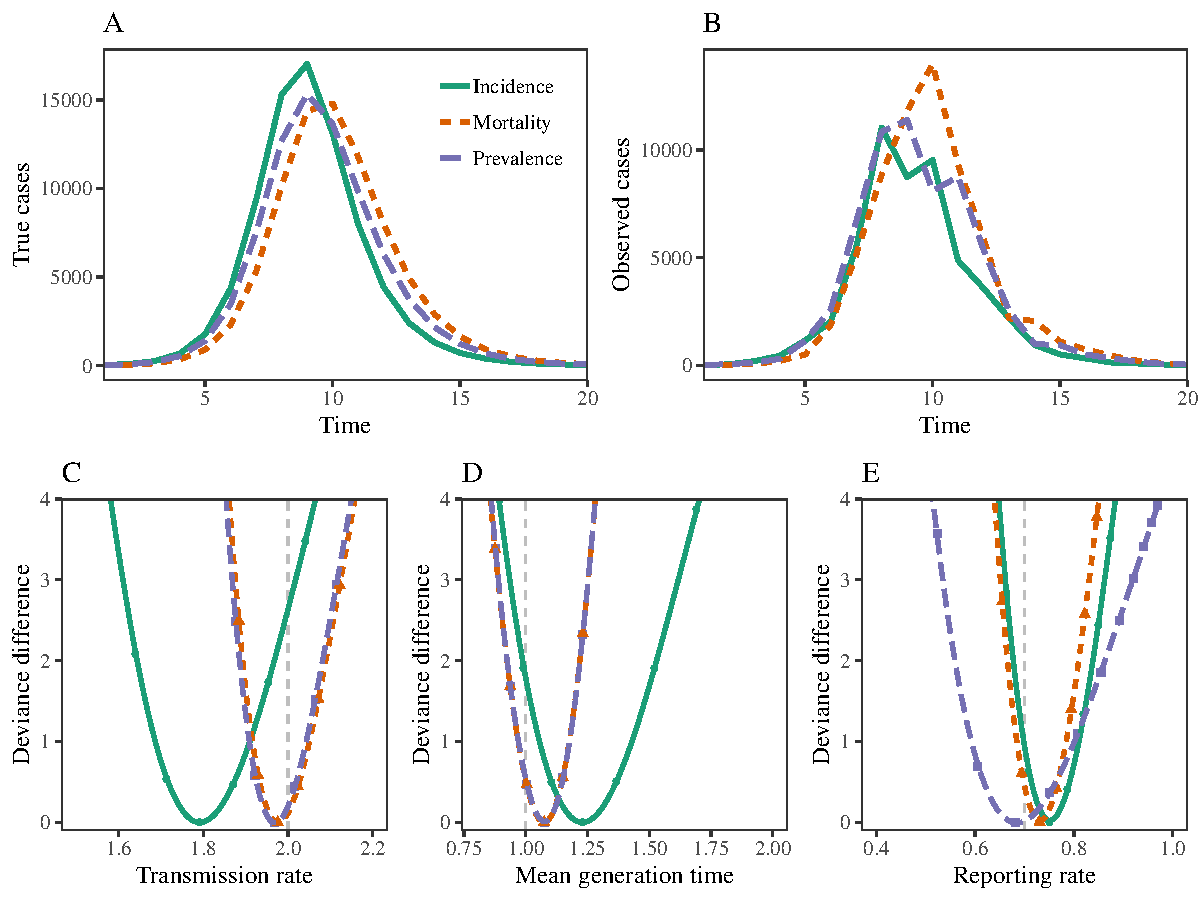
\includegraphics[width=\textwidth]{../figure/compare_profile_likelihood.pdf}
\caption{
\textbf{Comparison of incidence, prevalence, and mortality from dynamical and estimation perspective.}
A: dynamics of incidence, mortality and prevalence of the SIR model for a single outbreak (no natural birth/death and fixed transmission rate) when mean generation time ie equal to reporting period.
The parameters and initial conditions are $\beta = 2$, $\gamma = 1$, $N = 1 \times 10^5$, $I(0) = 10$, and $S(0) = N - 10$.
B: dynamics of incidence, mortality and prevalence of the SIR model with sinusoidal transmission rate ($\beta(t) = b_0 (1 + b_1 \cos (2 \pi t/26))$) when mean generation time ie equal to reporting period.
The parameters and initial conditions are $b_0 = 500/26$, $b_1 = 0.15$, $\gamma = 1$, $\mu = 1/(50 \times 26)$, $N = 5 \times 10^6$, $I(0) = 0.0001 N$, $S(0) = 0.05 N$.
C, D, E: deviance difference (profile likelihood minus the maximum likelihood) of each parameters when incidence, mortality, and prevalence are fit to same time series using trajectory matching. 
Grey dashed line represents the true value.
} 
\label{fig:incidence}
\end{figure}

Even if incidence, mortality, and prevalence are expected to be exhibit similar dynamics other when reporting period is equal to mean generation time, it is important to distinguish them when we are estimating underlying parameters of the SIR model, especially when mean generation time $1/\gamma$ is not exactly known.
To demonstrate this idea, we first simulate an epidemic time series representing prevalence over time by solving the SIR model numerically and calculating prevalence, $I(t)$, for 20 reporting periods, where reporting period is equal to the mean generation time. Then, we draw a beta-binomial random variable at each time step with a reporting rate of 70\% and an overdispersion parameter of 10.
Using this time series, we try to estimate four parameters -- transmission rate $\beta$, recovery rate $\gamma$, reporting rate $\rho$, and an initial number of infected individuals $I(0)$ -- by treating the same time series as if it were incidence, mortality, and prevalence report (\fref{incidence}).

We find that fitting prevalence and mortality curves to the same time series yields almost identical estimates of the transmission rate $\beta$ and the recovery rate $\gamma$ (as well as related uncertainty in the estimates) whereas fitting incidence and mortality curves to the same time series yields consistent estimates of the reporting rate $\rho$  (as well as related uncertainty in the estimates).
As mortality is approximately a lagged reflection of prevalence regardless of reporting period (reported mortality case at time $t$ is approximately equal to $\rho \gamma I(t-\tsub{t}{rep}) \tsub{t}{rep}$), 
it is possible to generate a mortality curve that matches its corresponding prevalence curve by adjusting the reporting rate $\rho$.
This explains why estimates of dynamical parameters, $\beta$ and $\gamma$, are similar whether we treat the same time series as prevalence or mortality.
On the other ahnd, incidence report no longer matches prevalence report when reporting period is not equal to the mean generation time (i.e., when $\gamma$ is being estimated); therefore, fitting incidence curve yields a different estimate of the dynamical parameters, $\beta$ and $\gamma$, from fitting mortality or prevalence curves.
Fitting incidence and mortality curve yields similar estimates of the reporting rate $\rho$ because they both contain equivalent information about the final size of an epidemic: total \emph{true} incidence and total \emph{true} mortality is equal to the final size of an epidemic.

Even when mean generation time is exactly known, we find that estimates of transmission rate $\beta$ and reporting rate $\rho$ depends on our assumptions about the data.
We find that fitting mortality and prevalence yields consistent estimates of both $\beta$ and $\rho$ in this case, whereas fitting incidence yields similar but still different estimates.
Treating incidence report as prevalene report (and vice versa) should be avoided.

\swp{Say something more}

\subsection{Susceptible reconstruction}

One of the main assumptions behind the TSIR model is that the dynamics susceptible population $S_t$ must be known.
Assuming that all newborn infants become infected eventually, it is possible to recover the reporting rate, $\rho_t$, as well as the dynamics of the susceptible population as a deviation from its mean, $Z_t = S_t - \bar{S}$, by fitting a regression model to between cumulative births and cumulative cases: 
\begin{equation}
\sum_{t=1}^N B_t = \sum_{t=1}^N \frac{C_{t+1}}{\rho_{t+1}} + Z_{t+1} - Z_1,
\end{equation}
where $C_t$ is the number of observed cases. 
Then, the mean susceptible population $\bar S$ can be estimated using profile likelihood with the TSIR regression.

While this method of reconstructing the susceptible dynamics has been successfully used with the TSIR method, 
several questions remain to be answered.
First, how sensitive is our inference to regression methods?
Second, does $Z_t$ represent deviation from the overall population mean $\bar{S}$ or from some sort of moving average (assuming that population changes over time)?
Likewise, how does changes in population size or reporting rate over time affect our estimate of $\rho_{t+1}$ or $Z_t$?
Finally, how do assumptions about the population size affect estimate of the transmission rate?

\begin{figure}
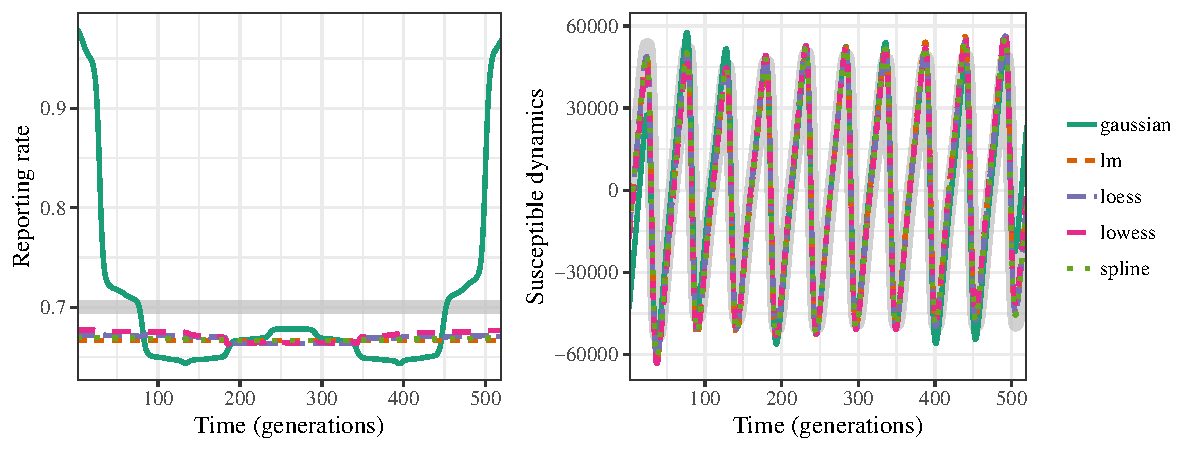
\includegraphics[width=\textwidth]{../figure/susceptible_reconstruction_tsir.pdf}
\caption{
\swp{TODO}
}
\label{fig:tsirrecon}
\end{figure}

We first simulate an epidemic using the continuous deterministic SIR model for 10 years and apply 5 different regression models available from the \texttt{tsiR} package to test their ability to infer reporting rate and susceptible dynamics (\fref{transmission}).
We find that estimates of transmission rates are highly sensitive to regression methods.
The gaussian regression is particularly inaccurate in boundaries.
Other methods provide similar estimates.
In general, estimates of susceptible dynamics appear to be robust regardless of the regression method.

\begin{figure}
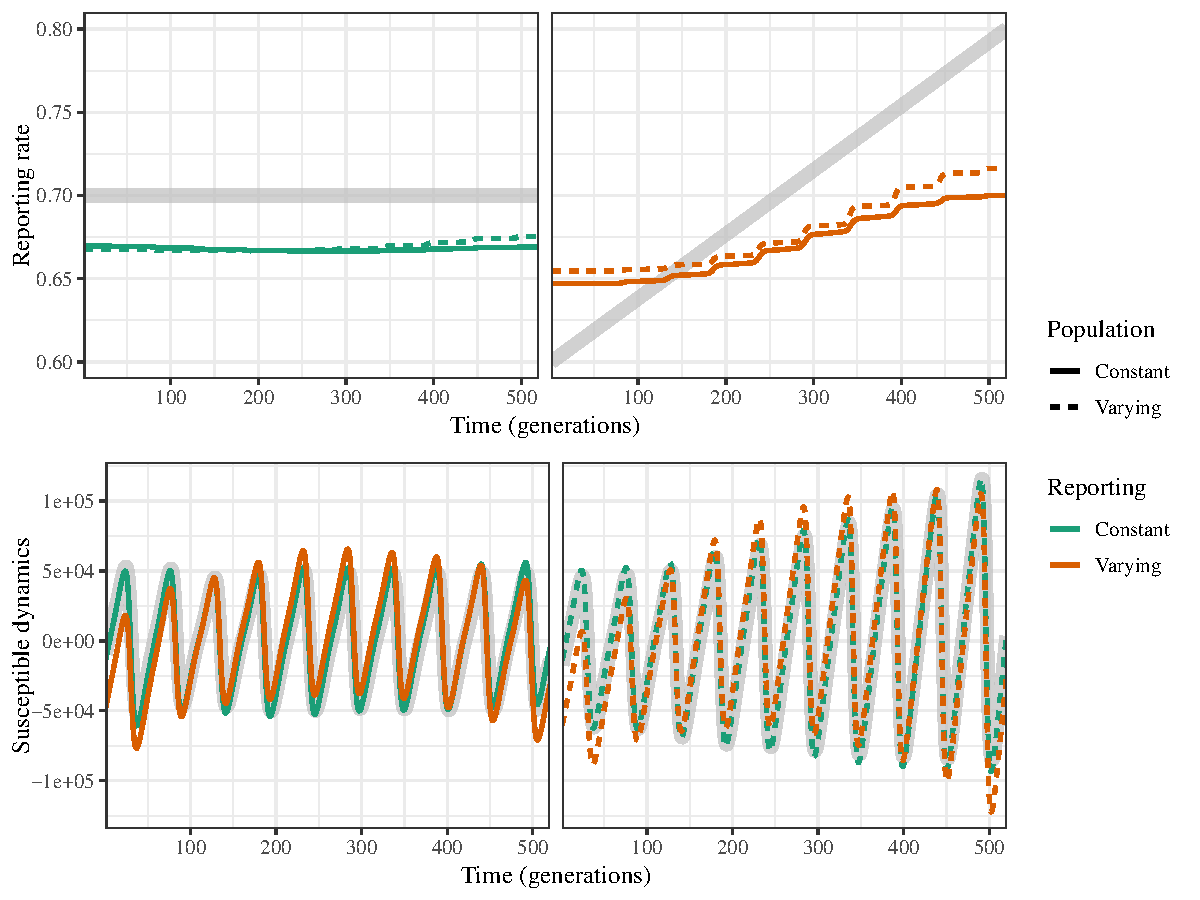
\includegraphics[width=\textwidth]{../figure/susceptible_reconstruction_compare.pdf}
\caption{
\swp{TODO}
}
\label{fig:tsircomp}
\end{figure}

Then, we compare estimates of susceptible dynamics and reporting rate under different scenarios (\fref{tsircomp}).
We allow for population size to stay constant or increase over time and also allow for reporting rate to stay constant or increase over time; these combinations yields 4 different scenarios.
We find that estimating time-varying reporting rate is difficult.
We also find that $Z_t$ estimated form regression better matches $S_t - \bar{S}$ rather than $S_t - \sigma N$, i.e., any long term dynamics in the susceptible population is captured in $Z_t$.

\subsection{Density dependence}

In continuous time SIR model, density dependence of the infection process is implicit in the nonlinear infection term, $\beta S I/N$.
In discrete time SIR models, density dependence must be accounted for explicitly.
The most common way to achieve this is to approximate the probability of infection a hazard: $1- \exp(- \phi \Delta t)$ where $\phi = \beta I/N$ is the force of infection.
This term accounts for increasing competition among infected individuals to find a susceptible host, which results in saturation in the probability of infection.

On the other hand, the TSIR model assumes that the probability of infection follows a power function of previous incidence: $\beta i^\alpha/N$, where $\alpha$ has been referred to as the correction factor for heterogeneity or discretization of a continuous model \citep{glass2003interpreting}.
\cite{glass2003interpreting} further derived an analytical expression for the optimal value of $\alpha$ as a function of birth rate and the basic reproductive number by comparing the second order Taylor expansion of the TSIR model to that of a continuous time model;
based on their approximation, 

Instead, interpreting $\alpha$ as the strength of density dependence, in line with our previous argument,  



\subsection{Estimates}



\section{Discussion}

\section{Data}

\section{TSIR model}

\subsection{Probability of infection}

The TSIR model assumes that probability of infection is a nonlinear function of prevalence: $\beta I^\alpha/N$.
This contrasts with the linear assumption of the Euler approximation ($\beta I/N$) or the exponenital assumption of the hazard-based approximation ($1 - \exp(- \beta I/N)$).
Inclusion of the parameter $\alpha$ has been previously attributed to heterogeneity in the population or changes from continuous to discrete time model.
However, there is still a room for clearer understanding of the actual role of the parameter $\alpha$:
for example, a few studies recognize that the estimated $\alpha$ does not always correspond to the best predictive $\alpha$ and resorted to assuming $\alpha = 0.97$.

Glass et al derived an analytical expression for optimal values of $\alpha$ by comparing the changes in the infected population at equilibrium using a second order Taylor expansion. 
Based on their approximation, optimal value of $\alpha$ equals 1 when there is no birth term.
Instead, when we rewrite the TSIR model as 
\begin{equation}
\log \left(\frac{I_{t+1}}{S_t}\right) = \log\left(\frac{\beta I_t^\alpha}{N_t}\right) + \epsilon_t.
\end{equation}
it becomes much clearer that the TSIR model is trying to match the log probability of infection (when an epidemic is ongoing, changes in the susceptible population $S_t$ through natural birth or death is negeligible over a generation, and $I_{t+1}/S_t$ can be interpreted as the probability of infection over a generation). 
Then, we almost always expect $\alpha$ to be less than one because we expect the probability of infection (i.e., probability of finding a new host) to experience density dependence.

Though the difference in the interpretation of $\alpha$ is subtle, this perspective allows us to derive a useful connection between the discrete-time model and the continuous-time model.
A naive estimate of basic reproductive number from the TSIR model is $\beta$.
However, as discussed earlier, we often prefer to use hazard-based approach to approximate the continuous-time model. 
Then, we can find $\hat \beta$ such that $1 - \exp(-\hat\beta I/N)$ matches $\beta I^\alpha/N$ and use $\hat \beta$ as our estimate of the basic reproductive number instead.
A simple way to match two functions is to match their values at the mean observed incidence.
This corrections reduces bias in the estimate of the reproductive number by a large amount.

\subsection{Process model}

The TSIR model is often associated with three different process models: deterministic ($I_{t+1} = \beta_t S_t I_t^\alpha/N$), poisson ($I_{t+1} \sim \mathrm{Poisson}(\beta_t S_t I_t^\alpha/N)$), and negative binomial ($I_{t+1} \sim \mathrm{NB}(\beta_t S_t I_t^\alpha/N, I_t)$).


\subsection{Susceptible reconstruction}



\pagebreak


\section{Appendix}

\subsection{Equivalence of incidence, mortality, and prevalence}

First, recall that mortality case can be written as
\begin{equation}
\int_{t-\tsub{t}{rep}}^{t} \gamma I ds.
\end{equation}
When reporting period is equal to mean generation time, i.e., $\tsub{t}{rep} = 1/\gamma$, 
it follows that:
\begin{equation}
\int_{t-\tsub{t}{rep}}^{t} \gamma I ds \approx \gamma I(t-\tsub{t}{rep}) \tsub{t}{rep} = I(t-\tsub{t}{rep})
\end{equation}
Likewise, we can derive a similar relation for incidence:
\begin{equation}
\begin{aligned}
I(t+\tsub{t}{rep}) &= I(t) + \int_{t}^{t+\tsub{t}{rep}} \frac{dI(s)}{ds} ds\\
&= I(t) + \int_{t}^{t+\tsub{t}{rep}} \beta(s) S \frac{I}{N} ds - \int_{t}^{t+\tsub{t}{rep}}\\
&\approx \int_{t}^{t+\tsub{t}{rep}} \beta(s) S \frac{I}{N} ds
\end{aligned}
\end{equation}
Here, we assumed that individuals leaving infected class $I$ from natural mortality is negligible over the reporting period.

\swp{TODO}


\section{Fitting continuous models}

\subsection{Gradient matching}

\begin{figure}[t]
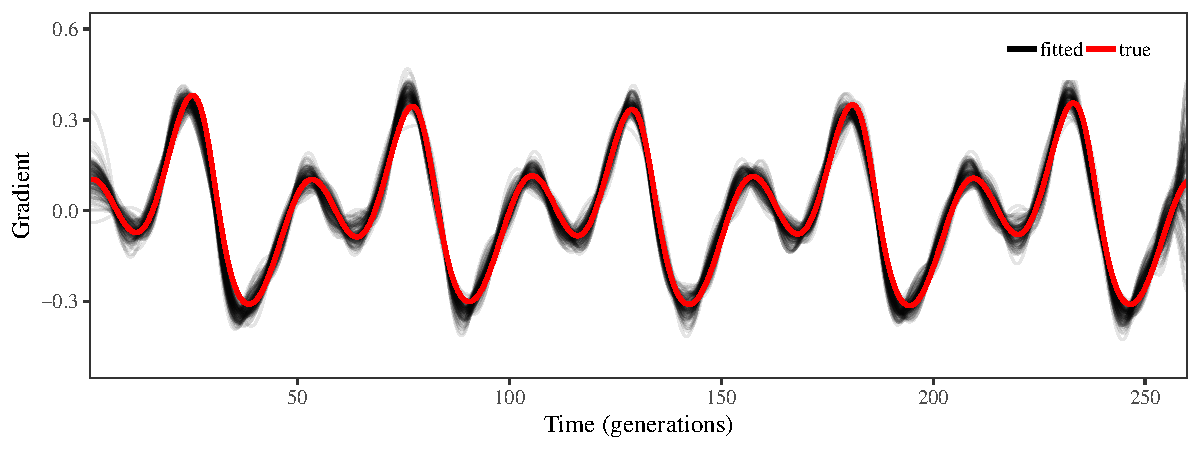
\includegraphics[width=\textwidth]{../figure/gradient_matching_sinusoidal.pdf}
\caption{This is not a caption.}
\end{figure}

Conditions:
\begin{itemize}
	\item See Jost and Ellner (???)
	\item sampled sufficiently
	\item not too much error
	\item Brunel Parameter estimation of ODE’s via nonparametric estimators
\end{itemize}


%% read pomp-Astic somewhere

\subsection{Spectral matching}

What is this? Read Reuman et al. 2006
%% https://www.pnas.org/content/pnas/103/49/18860.full.pdf


\bibliography{thesis}

\pagebreak

\section{Appendix}

\subsection{Derivation of growth rate in discrete-time SIR model}


Derivation:
\begin{equation}
\begin{aligned}
S_{t+\Delta t} &= S_t - S_t (1- \exp(-\beta I_t \Delta t/N))\\
I_{t+\Delta t} &= S_t (1- \exp(-\beta I_t \Delta t/N)) + I_t - I_t (1- \exp(-\gamma \Delta t))
\end{aligned}
\end{equation}
Assuming tat $S_t$ is approximately equal to $N$, we get
\begin{equation}
I_{t+\Delta t} = N_t (1- \exp(-\beta I_t \Delta t/N)) + I_t \exp(-\gamma \Delta t)
\end{equation}
When $I_t \approx 0$, $\exp(-\beta I_t \Delta t/N) \approx 1 - \beta I_t \Delta t/N$ and so
\begin{equation}
\begin{aligned}
I_{t+\Delta t} &\approx  I_t \beta \Delta t + I_t \exp(-\gamma \Delta t)\\
&= I_t (\beta \Delta t + \exp(-\gamma \Delta t))
\end{aligned}
\end{equation}
Substituting $\hat{\gamma}$, we get
\begin{equation}
I_{t+\Delta t} = I_t \left(1 + \beta \Delta t - \frac{\Delta t}{\mu}\right),
\end{equation}
Therefore,
\begin{equation}
I_{t} = I_0 \left(1 + \beta\Delta t - \frac{\Delta t}{\mu}\right)^{t/\Delta t}
\end{equation}
and the initial growth rate is given by
\begin{equation}
r = \frac{1}{\Delta t} \log \left(1 + \beta \Delta t - \frac{\Delta t}{\mu}\right).
\end{equation}




\subsection{Probability of infection}

In both the TSIR model and the hazard-based model, transition from the susceptible comparment, $S$, to the infected compartment, $I$, is represented as a product of number of susceptible individuals and probability of infection between two time steps $t$ and $t + \Delta t$.
The TSIR model assumes that the probability of infection is a linear function of prevalence $I_t$.
This formulation is based on the Euler approximation to the solution of the ordinary differential equation.
On the other hand, the hazard-based model assumes that the probability of infection is an inverse exponential function of prevalence $I_t$.
Besides their differences in the relationship between prevalence and probability of infection, there are two more assumptions that we need to consider: (1) force of infection remains constant over two time steps and (2) new susceptible individuals have zero probability of infection between the two time steps.



\subsection{Infectious period}

Geometric distribution with probability of $1-\exp(-\gamma \Delta t)$ and unit of $\Delta t$.
Then, mean infectious period and generation interval is given by 
\begin{equation}
\frac{\Delta t}{1-\exp(-\gamma \Delta t)}.
\end{equation}
An important but often overlooked component is the variance of the distribution.
Squared coefficient of variation for this distribution is equal to $\exp(-\gamma \Delta t)$, which necessarily depends on pre-specified time-step $\Delta t$.
If we want to match the mean of the distribution to a fixed value $\mu$ regardless of our choices of $\Delta t$, we obtain 
\begin{equation}
\hat \gamma = - \frac{1}{\Delta t} \log\left(1 - \frac{\Delta t}{\mu}\right)
\end{equation}
Then,
\begin{equation}
\mathrm{CV}_{\tiny\textrm{Infectious period}}(\Delta t)^2 = 1 - \frac{\Delta t}{\mu}.
\end{equation}

We expect changes in variation in infectious period to affect variation in stochstic realizations.

This means that the relationship between $r$ and $\mathcal R$ changes.
For this generation-interval distribution, we have
\begin{equation}
\mathcal R = 1 + \frac{\exp(r) -1}{(1-\exp(-\gamma \Delta t)) }
\end{equation}
Substituting 
\begin{equation}
r = \frac{1}{\Delta t} \log \left(1 + \beta \Delta t - \frac{\Delta t}{\mu}\right),
\end{equation}
as well as $\hat \gamma$, we get
\begin{equation}
\mathcal R = 1 + \frac{\mu}{\Delta t} \left(1 + \beta \Delta t - \frac{\Delta t}{\mu}\right)^{1/\Delta t}
\end{equation}
Then, we can obtain a relationship between $\mathcal R$ of a discrete-time system and that of a corresponding continuous time system, assuming that contact rate $\beta$ and mean generation-time $\mu$ are the same:
\begin{equation}
\mathcal R_{\tiny \textrm{discrete}} = 1 + \frac{\mu}{\Delta t} \left(1 + \frac{(\mathcal R_{\tiny \textrm{continuous}}  - 1) \Delta t }{\mu}\right)^{1/\Delta t}
\end{equation}

On the other hand, we may want to match choose $\beta$ and $\mu$ to match true $r$ and $\mathcal R$.



\end{document}
